\section{Referencia de la Clase Inventario\-View}
\label{classInventarioView}\index{InventarioView@{InventarioView}}
Muestra y administra la ventana con los datos de un inventario.  


{\tt \#include $<$inventarioview.h$>$}

Diagrama de herencias de Inventario\-View\begin{figure}[H]
\begin{center}
\leavevmode
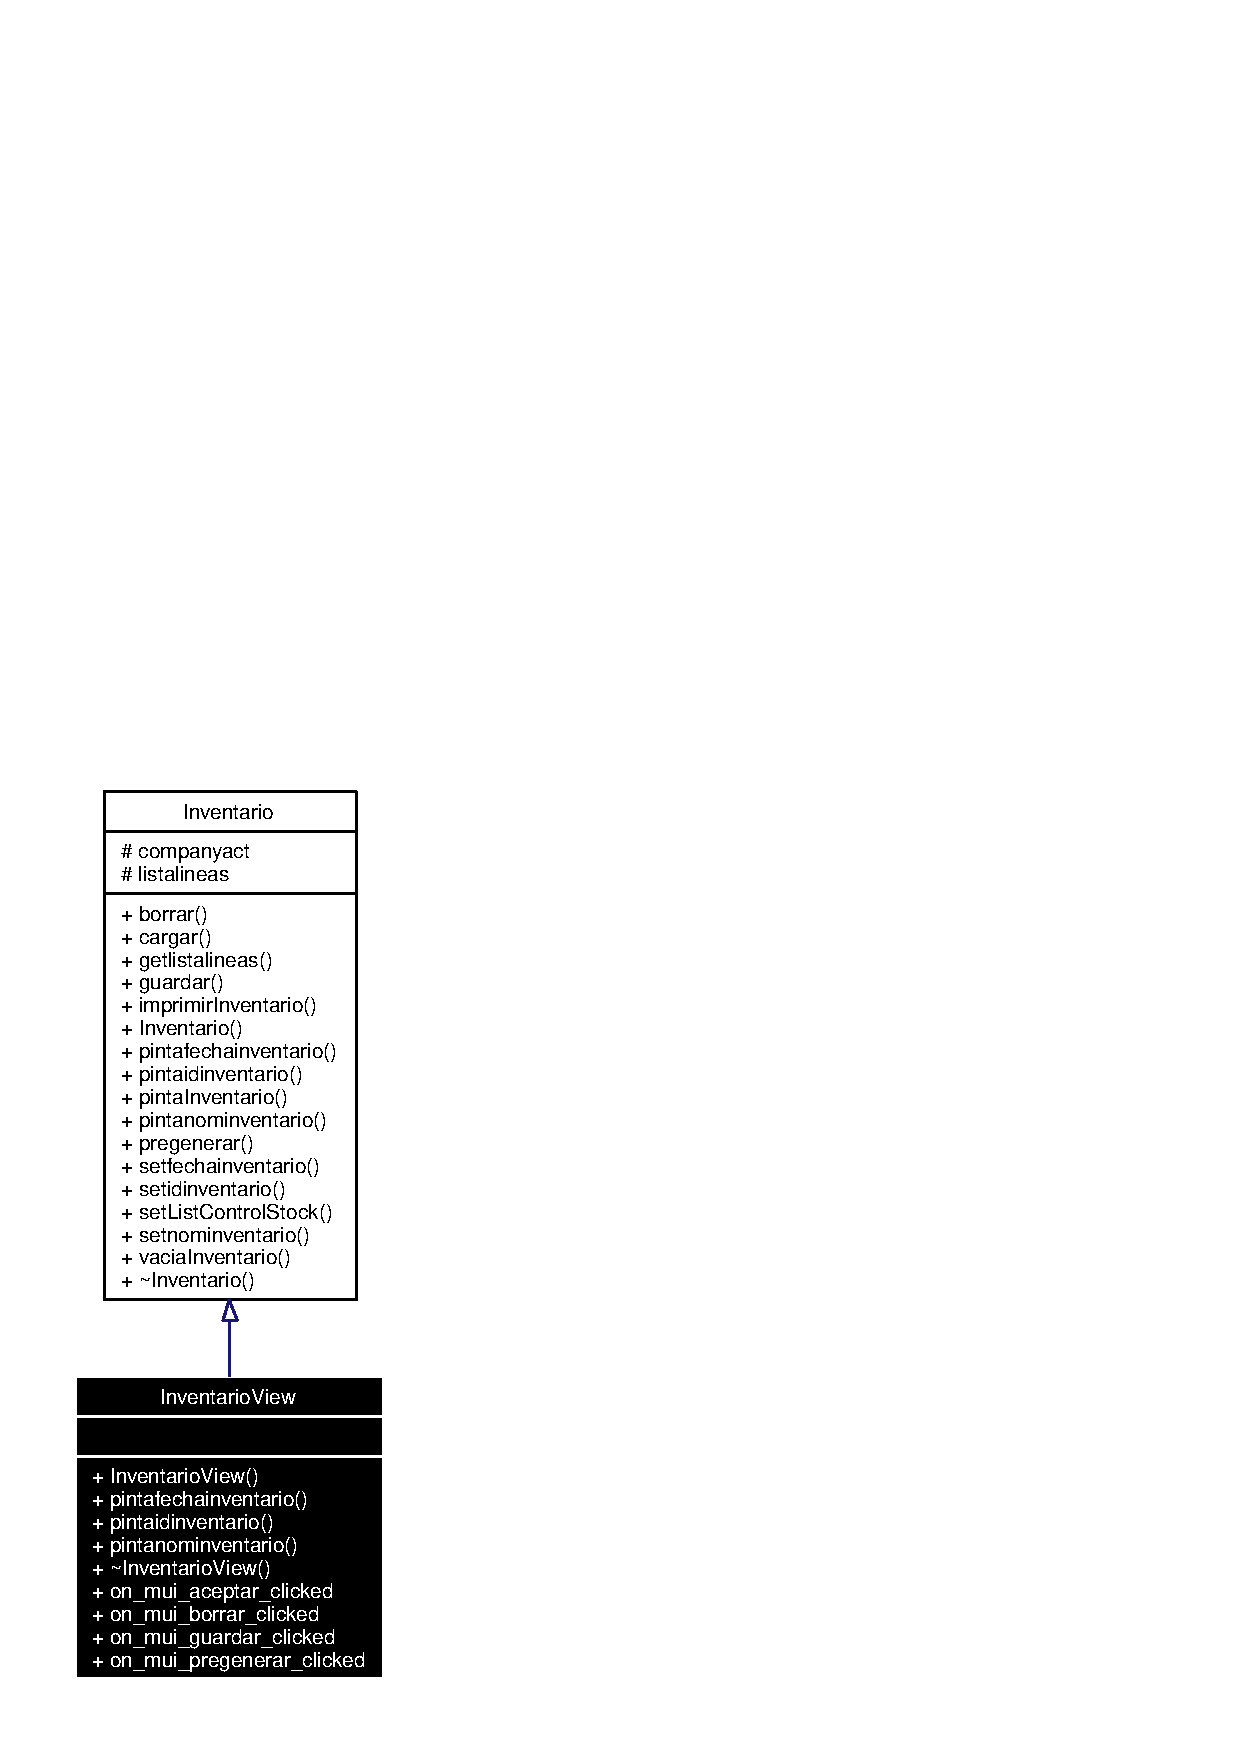
\includegraphics[width=92pt]{classInventarioView__inherit__graph}
\end{center}
\end{figure}
Diagrama de colaboraci\'{o}n para Inventario\-View:\begin{figure}[H]
\begin{center}
\leavevmode
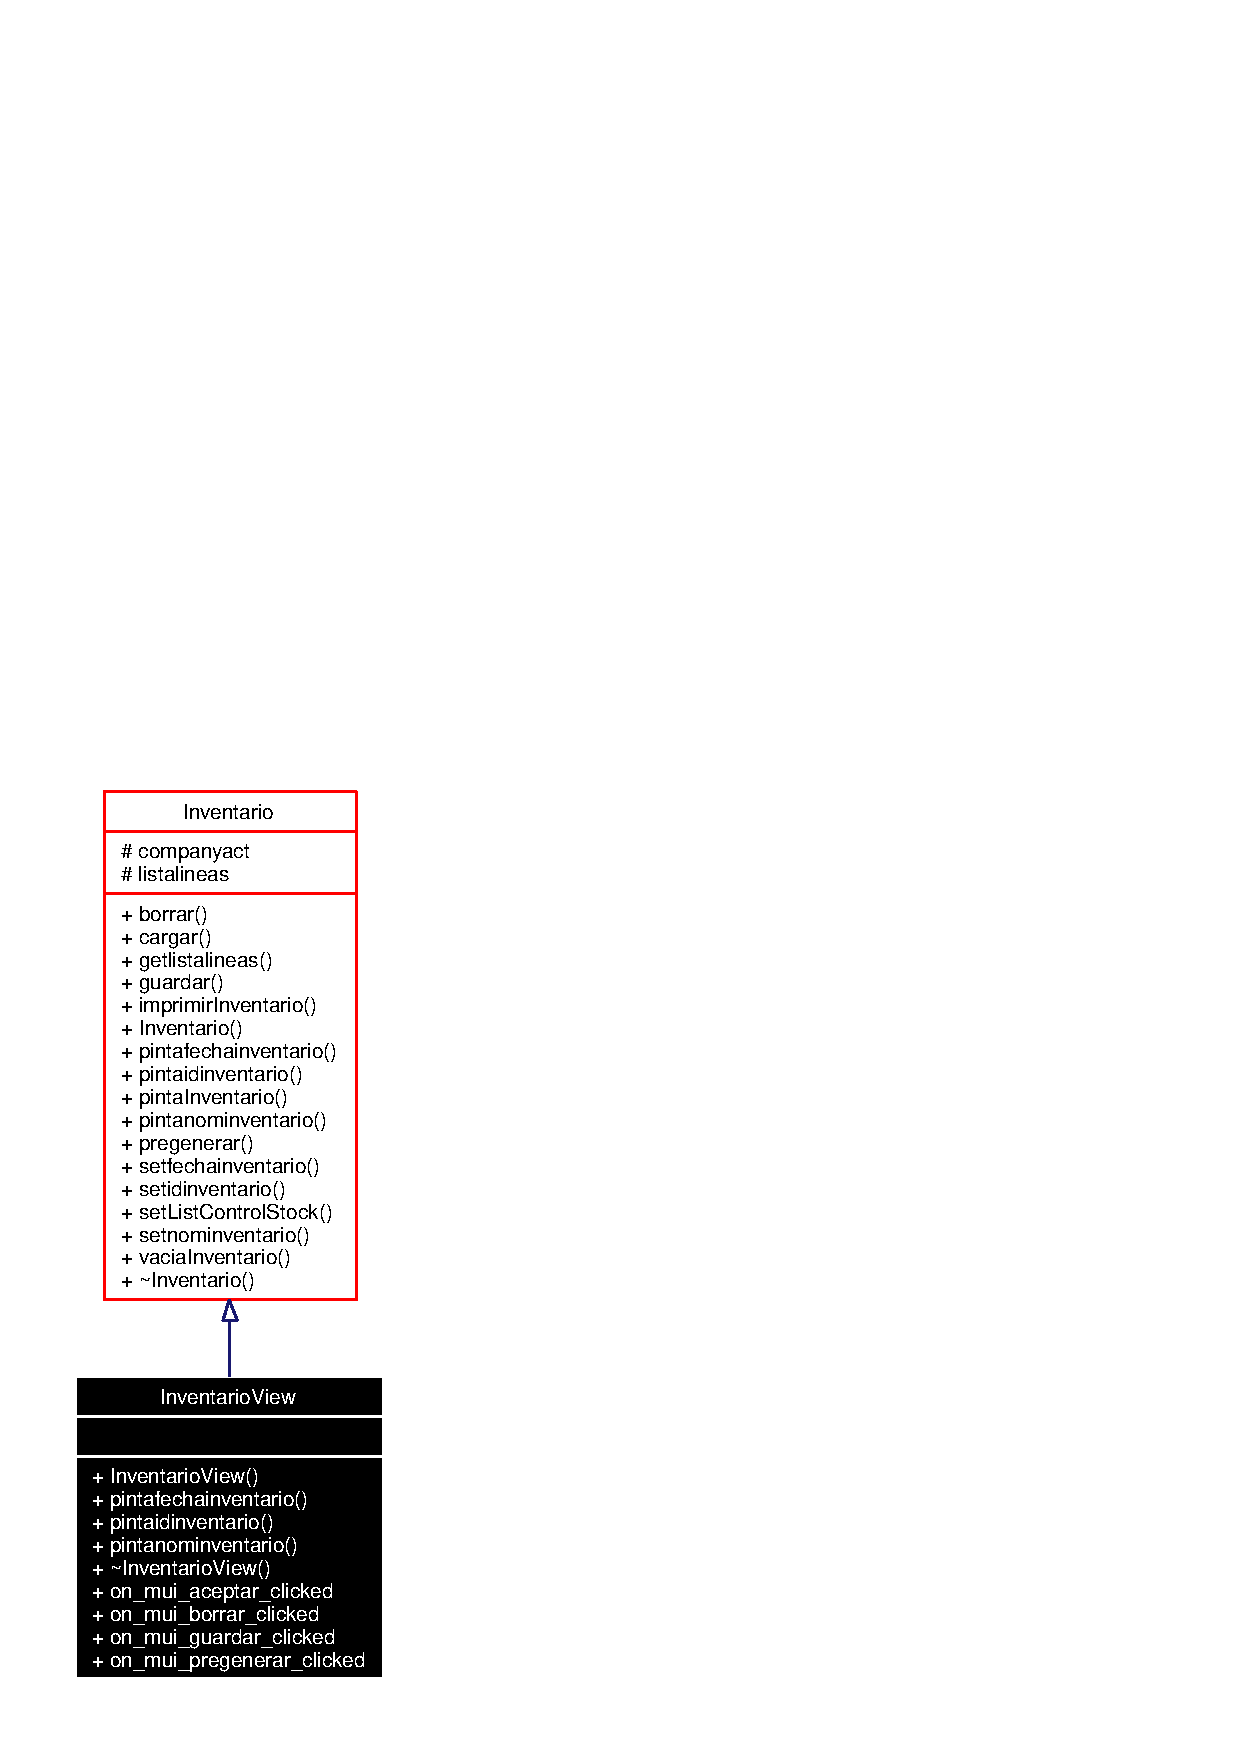
\includegraphics[width=92pt]{classInventarioView__coll__graph}
\end{center}
\end{figure}
\subsection*{Slots p\'{u}blicos}
\begin{CompactItemize}
\item 
virtual void {\bf on\_\-mui\_\-aceptar\_\-clicked} ()\label{classInventarioView_i0}

\item 
virtual void {\bf on\_\-mui\_\-borrar\_\-clicked} ()\label{classInventarioView_i1}

\begin{CompactList}\small\item\em Esta funcion se ejecuta cuando se ha pulsado sobre el boton de borrar. \item\end{CompactList}\item 
virtual void {\bf on\_\-mui\_\-guardar\_\-clicked} ()\label{classInventarioView_i2}

\item 
virtual void {\bf on\_\-mui\_\-pregenerar\_\-clicked} ()\label{classInventarioView_i3}

\end{CompactItemize}
\subsection*{M\'{e}todos p\'{u}blicos}
\begin{CompactItemize}
\item 
{\bf Inventario\-View} ({\bf company} $\ast$, QWidget $\ast$parent=0)
\item 
void {\bf pintafechainventario} (QString id)\label{classInventarioView_a1}

\item 
void {\bf pintaidinventario} (QString)\label{classInventarioView_a2}

\item 
void {\bf pintanominventario} (QString id)\label{classInventarioView_a3}

\end{CompactItemize}


\subsection{Descripci\'{o}n detallada}
Muestra y administra la ventana con los datos de un inventario. 



\subsection{Documentaci\'{o}n del constructor y destructor}
\index{InventarioView@{Inventario\-View}!InventarioView@{InventarioView}}
\index{InventarioView@{InventarioView}!InventarioView@{Inventario\-View}}
\subsubsection{\setlength{\rightskip}{0pt plus 5cm}Inventario\-View::Inventario\-View ({\bf company} $\ast$ {\em comp}, QWidget $\ast$ {\em parent} = {\tt 0})}\label{classInventarioView_a0}


Usurpamos la identidad de mlist y ponemos nuestro propio widget con sus cosillas. 

La documentaci\'{o}n para esta clase fu\'{e} generada a partir de los siguientes archivos:\begin{CompactItemize}
\item 
inventarioview.h\item 
inventarioview.cpp\end{CompactItemize}
